\section{Methods of Classification}
\begin{frame}
	\begin{center}
	%{\color{-green!15!yellow}
	\Large{Methods of Classification}
	%}
	\end{center}
\end{frame}

\subsection{Logistic Regression}

\begin{frame}
	\frametitle{Logistic Regression}
	\begin{columns}
	\column[c]{0.4\textwidth}
	\begin{itemize}
		\item Builds score out of weighted features.
		\item Uses score in logistic function.
		\item Predicts the \emph{probability} of test data being part of a class.
	\end{itemize}
	\column[c]{0.6\textwidth}
	\begin{figure}
	\includegraphics[width=\linewidth]{images/logisticf}
	\caption{\raggedleft The standard logistic function \cite{logfuWiki}}
	\end{figure}
	\end{columns}
\end{frame}

\subsection{K Nearest Neighbor}

\begin{frame}
	\frametitle{K Nearest Neighbor}
	Compare new data point directly to \emph{nearest} training data points.
\end{frame}

\begin{frame}
	\frametitle{K Nearest Neighbor}
	\begin{figure}
	\includegraphics[width=0.7\textwidth]{images/knn0}
	\caption{Initializing kNN}
	\end{figure}
\end{frame}

\begin{frame}
	\frametitle{K Nearest Neighbor}
	\begin{figure}
	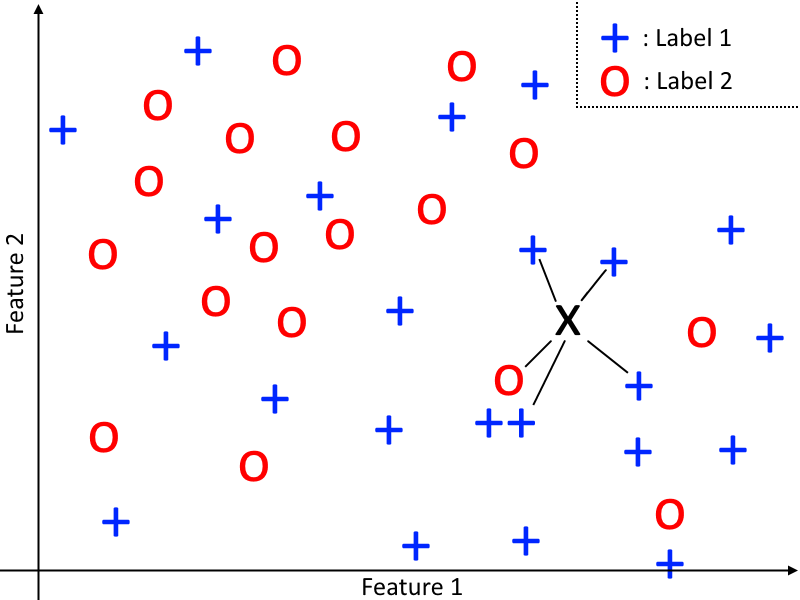
\includegraphics[width=0.7\textwidth]{images/knn1}
	\caption{Prediction in kNN (1)}
	\end{figure}
\end{frame}

\begin{frame}
	\frametitle{K Nearest Neighbor}
	\begin{figure}
	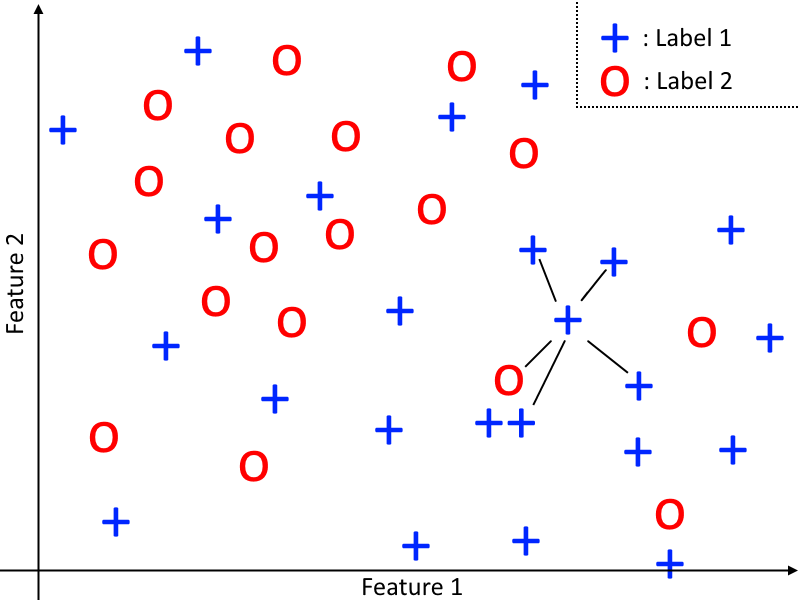
\includegraphics[width=0.7\textwidth]{images/knn2}
	\caption{Prediction in kNN (2)}
	\end{figure}
\end{frame}



\subsection{XGBoost}
\begin{frame}
	\frametitle{XGBoost}
	\begin{itemize}
		\item Gradient Boosting classifier developed by Tianqi Chen.
		\item Shared early with other participants and grew popular.
		\item Was acknowledged with the \emph{HEP meets ML Award}.\begin{itemize}
			\item Prediction performance
			\item Documentation
			\item CPU and memory demands
			\item simplicity/straightforwardness of approach
		\end{itemize}
	\end{itemize}
\end{frame}

\begin{frame}
	\frametitle{Boosting}
	\begin{columns}
	
	\column[c]{0.5\textwidth}
	\begin{tabular}{r l}
	\\\\
		$f_1(x)  = $ & $y - error$\\\\
		$error  = $ & $y - f_1(x)$\\\\
		$f_2(x)  = $ & $y - f_1(x)$\\\\
		$f_1(x)+f_2(x)  = $ & $y - error_2$\\\\
		\ldots
	\end{tabular}
		
	\column[c]{0.5\textwidth}
	\begin{block}{}
	We combine an ensemble of \emph{weak learners} $f_i(x)$ into one \emph{strong learner} $F(x)$.
	\end{block}
		
	\end{columns}
\end{frame}

\begin{frame}
	\frametitle{Gradient Boosting}
	
	\begin{columns}
	
	\column[c]{0.5\textwidth}
	\begin{tabular}{r l}
	\\\\
	square loss: $l =$ & $\sum\limits_{i}^{n} \frac{(f_i(x)-y)^2}{2}$
	\\\\
	$\frac{\partial l}{\partial f_1(x)}  = $ & $f_1(x)-y$\\\\
	$- \frac{\partial l}{\partial f_1(x)}  = $ & $y - f_1(x)$\\\\
	$- \frac{\partial l}{\partial f_1(x)}  = $ & $f_2(x)$
	\end{tabular}
	
	\column[c]{0.5\textwidth}
	\begin{block}{}
	Residuals can be interpreted as \emph{negative gradients}.\\ \vspace{4ex}
	If we fit \emph{weak learners} to \emph{negative gradients}, it allows to minimize the loss function using \emph{gradient descent}.
	\end{block}
	\end{columns}
	
	\vspace{4ex}
	One can show that a gradient boosting algorithm can be constructed for any loss function \cite{gradboost}.
\end{frame}

\begin{frame}
	\frametitle{XGBoost}
	\begin{center}
	Regularized objective function
	$$L=\sum\limits_{i} l(y_i,\hat{y}_i)+\sum\limits_{k} \Omega (f_k)$$
	\end{center}
	\begin{itemize}
		\item $l$ is any loss function.
		\item $\Omega(f_k)$ measures complexity of classifier $f_k$.
		\item As $L$ is minimized, so are $l$ and $\Omega$.
	\end{itemize}
\end{frame}

\begin{frame}
	\frametitle{XGBoost}
	\begin{center}
	\begin{figure}
		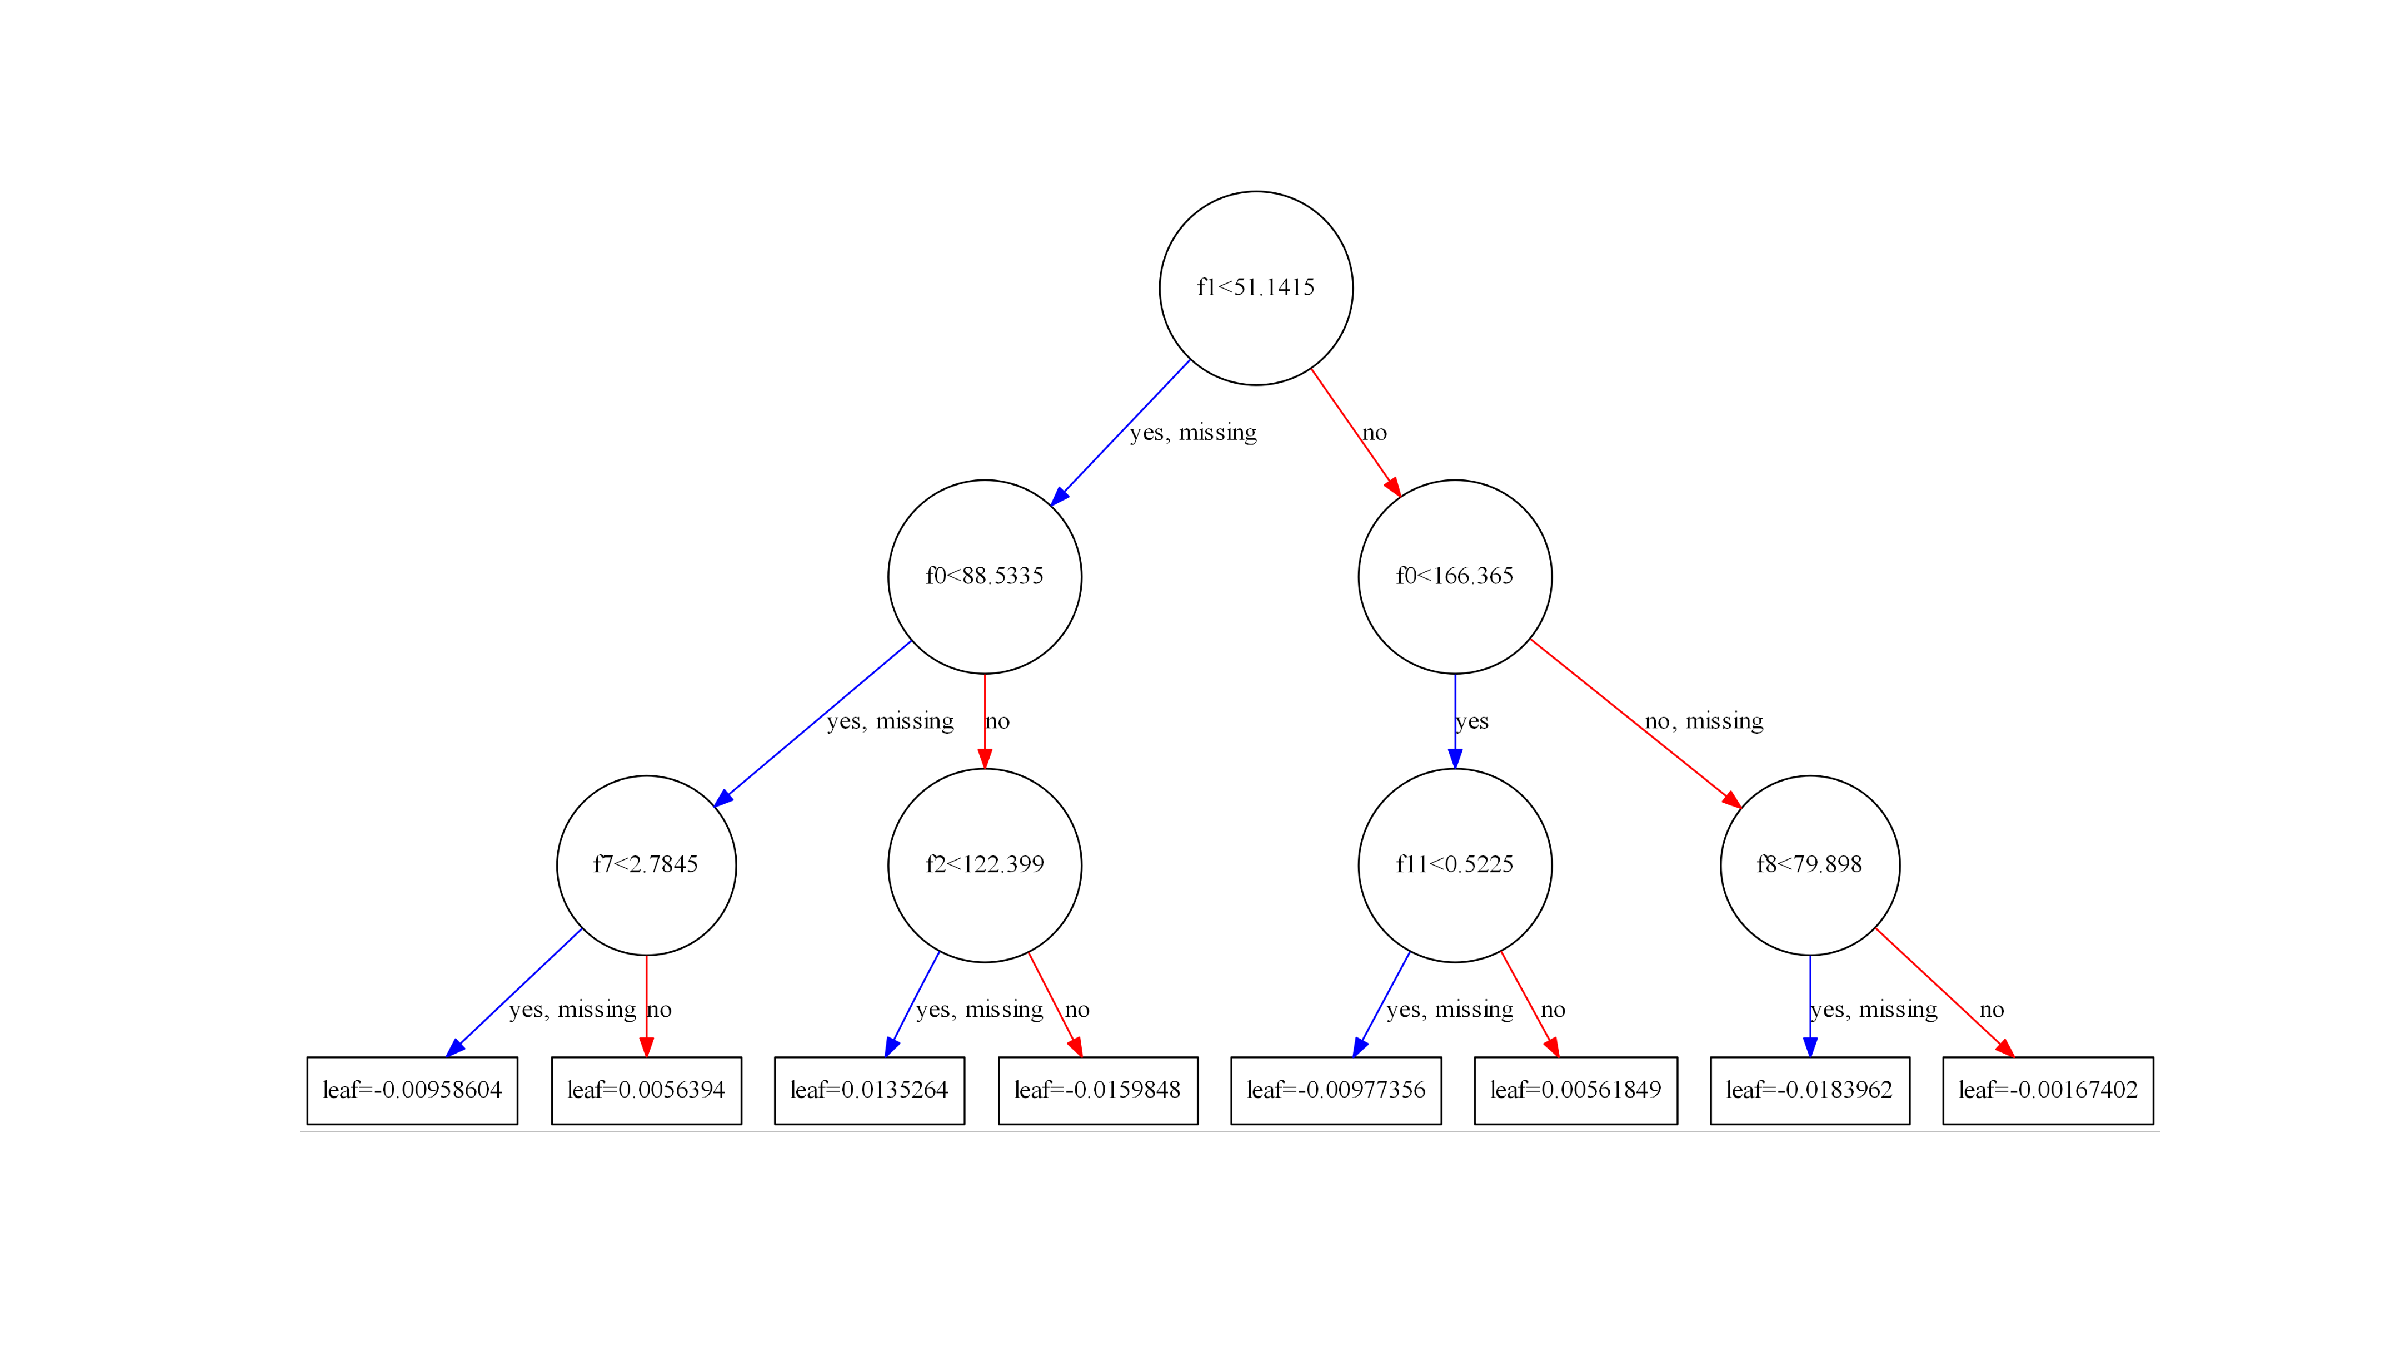
\includegraphics[trim=146 100 118 90, clip, width=\textwidth]{images/tree.pdf}
\caption{A decision tree generated by XGBoost.}
	\end{figure}
	\end{center}

\end{frame}